\documentclass[dcc,sol]{fcfmcourse}
\usepackage{teoria}
\usepackage[utf8x]{inputenc}
\usepackage{amsmath}
\usepackage{amsfonts,setspace}
\usepackage{listings}
\usepackage{color}
\usepackage{epstopdf}
\usepackage{multicol}
\setlength{\columnsep}{1cm}

\definecolor{pblue}{rgb}{0.13,0.13,1}
\definecolor{pgreen}{rgb}{0,0.5,0}
\definecolor{porange}{rgb}{0.9,0.5,0}
\definecolor{pgrey}{rgb}{0.46,0.45,0.48}

\lstset{language=Java,
  showspaces=false,
  showtabs=false,
  breaklines=true,
  showstringspaces=false,
  breakatwhitespace=true,
  commentstyle=\color{porange},
  keywordstyle=\color{pblue},
  stringstyle=\color{pgreen},
  basicstyle=\ttfamily,
  moredelim=[il][\textcolor{pgrey}]{$ $},
  moredelim=[is][\textcolor{pgrey}]{\%\%}{\%\%}
}

\newenvironment{codebox} {\small \ttfamily \obeylines \begingroup \setstretch{-2.4}} {\endgroup}

\title{Auxiliar 12 - Solución}
%\course[CC3001]{Algoritmos y Estructuras de Datos}
%\professor{Nelson Baloian}
%\professor{Patricio Poblete}
%\assistant{Manuel Cáceres}
%\assistant{Sebastián Ferrada}
%\assistant{Sergio Peñafiel}

% Si pasas el comando usedate a la clase, la fecha aparecerá bajo la lista de auxiliares.
% Puedes usar el formato de fecha por defecto de latex (y traducirla usando babel)
% o puedes escribir lo que quieras con el comando \date.
% \date{1 de Septiembre, 2015}


\begin{document}
\maketitle

\vspace{-1ex}

\begin{problems}

\problem \textbf{Caminos Mínimos}

\begin{enumerate}[1.]

\item Se inicializa el grafo con los pesos (texto azul) infinito para todos los nodos excepto el inicial que es 0.
\begin{center}
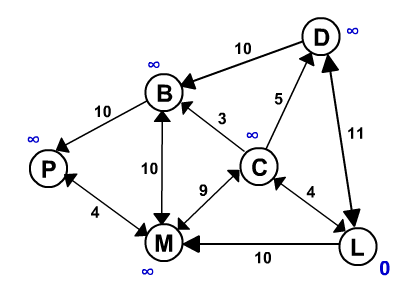
\includegraphics[scale=0.65]{dijkstra0001.png}
\end{center}

\item Se busca el nodo con peso menor no visitado, en este caso L y se actualiza el peso de todos sus vecinos.
\begin{center}
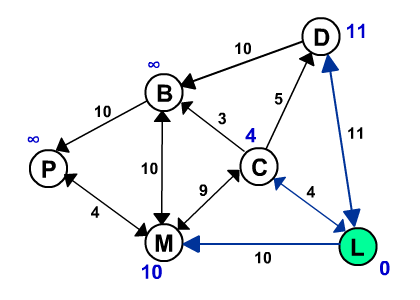
\includegraphics[scale=0.65]{dijkstra0002.png}
\end{center}

\item Se busca el nodo con peso menor no visitado, en este caso C y se actualiza el peso de todos sus vecinos excepto M que tiene un peso más bajo.
\begin{center}
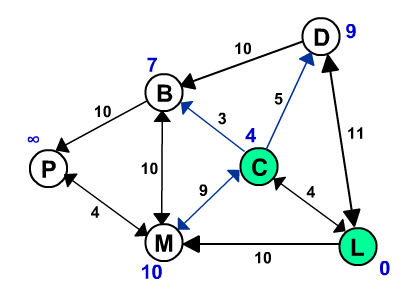
\includegraphics[scale=0.65]{dijkstra0003.png}
\end{center}

\item Se busca el siguiente nodo con peso menor no visitado, en este caso B y se actualiza el peso de todos sus vecinos excepto M que tiene un peso más bajo.
\begin{center}
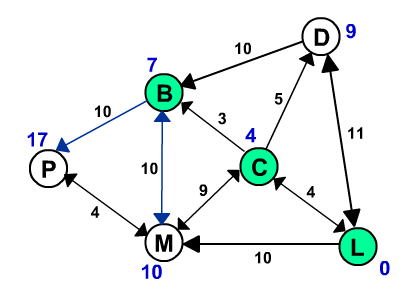
\includegraphics[scale=0.65]{dijkstra0004.png}
\end{center}

\newpage
\item Se busca el siguiente nodo con peso menor no visitado, en este caso D el cual no actualiza el valor de sus vecinos por estar ya visitados.
\begin{center}
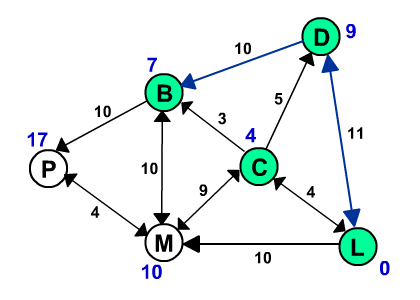
\includegraphics[scale=0.65]{dijkstra0005.png}
\end{center}

\item Se busca el siguiente nodo con peso menor no visitado, en este caso M el cual actualiza sólo el valor de P dado que es el unico no visitado.
\begin{center}
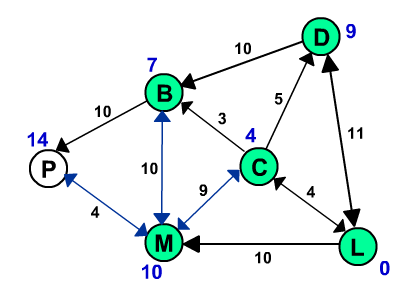
\includegraphics[scale=0.65]{dijkstra0006.png}
\end{center}

\newpage
\item Se busca el último nodo no visitado P, el cual no tiene vecinos por lo que no se actualizan valores.
\begin{center}
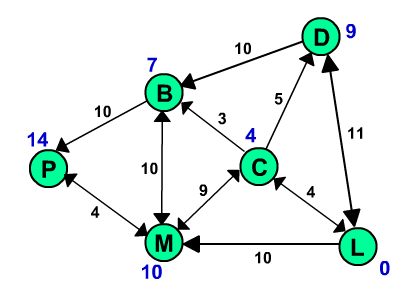
\includegraphics[scale=0.65]{dijkstra0007.png}
\end{center}

\item Al finalizar el peso resultante de los nodos indica el costo del camino mínimo desde L hasta cada uno de los nodos.

\end{enumerate}

Grafo B

\begin{enumerate}[1.]

\item Se inicializa el grafo con los pesos infinito para todos los nodos y 0 para el inicial.
\begin{center}
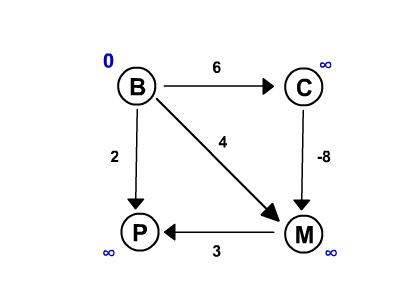
\includegraphics[scale=0.65]{dijkstra0008.png}
\end{center}

\newpage
\item Se busca el nodo con peso menor no visitado, en este caso B y se actualiza el peso de todos sus vecinos.
\begin{center}
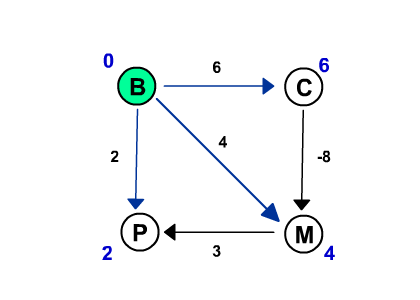
\includegraphics[scale=0.65]{dijkstra0009.png}
\end{center}

\item Se busca el siguiente nodo con peso menor no visitado, en este caso P que no tiene vecinos.
\begin{center}
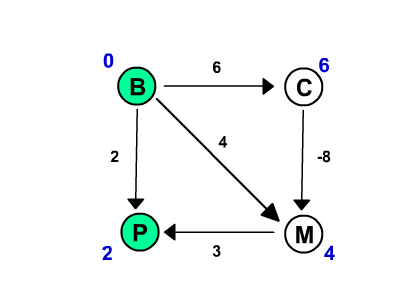
\includegraphics[scale=0.65]{dijkstra0010.png}
\end{center}

\newpage
\item Se busca el siguiente nodo con peso menor no visitado, en este caso M que no actualiza el valor de P porque ya esta visitado.
\begin{center}
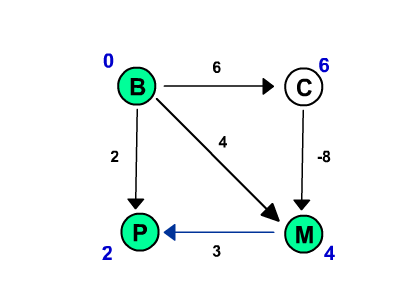
\includegraphics[scale=0.65]{dijkstra0011.png}
\end{center}

\item Se busca el último nodo no visitado C, el cual no actualiza el valor de sus vecinos porque ya están visitados.
\begin{center}
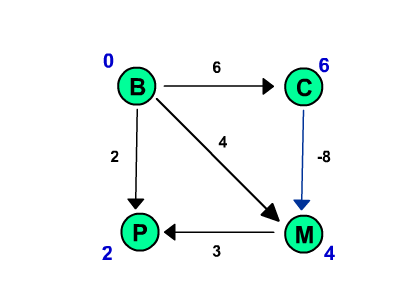
\includegraphics[scale=0.65]{dijkstra0012.png}
\end{center}

\item El estado final del algoritmo indica los costos de los caminos mínimos desde B a cualquier otro nodo, sin embargo el resultado es claramente incorrecto, por ejemplo el camino con menor costo de B a M es B-C-M el cual tiene costo -2. Esto se debe a que el algoritmo de Dijkstra toma como supuesto que el peso de todos los arcos es positivo.

\end{enumerate}

\newpage
\problem \textbf{Compresión (Huffman)}

Para cada texto se crea primero la tabla de frecuencias para cada símbolo según la cantidad de apariciones que tiene, luego se crea el trie mediante la agrupación de símbolos tal que su peso sea el menor posible, se itera hasta agregar todos los símbolos al árbol. Con el árbol listo se asigna 0 a la izquierda y 1 a la derecha y se obtiene la codificación de cada símbolo, finalmente se reemplaza el símbolo con su codificación siguiendo el camino en el árbol. Muchas veces el trie y la codificación no son únicas.

\begin{itemize}
\item AAABCBABBC \\

\begin{multicols}{2}
\begin{tabular}{|c|c|} \hline
Simbolo & Frecuencia  \\ \hline
A & 4/10 \\
B & 4/10 \\
C & 2/10 \\ \hline
\end{tabular}

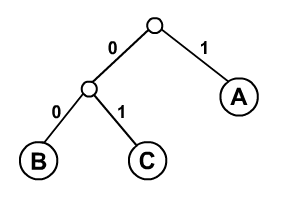
\includegraphics[scale=0.5]{trie1.png}
\end{multicols}

Texto comprimido: \texttt{1.1.1.00.01.00.1.00.00.01} \\

\item ABCBCAAACB \\

\begin{multicols}{2}
\begin{tabular}{|c|c|} \hline
Simbolo & Frecuencia  \\ \hline
A & 4/10 \\
B & 3/10 \\
C & 3/10 \\ \hline
\end{tabular}

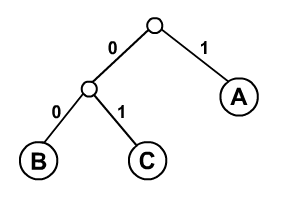
\includegraphics[scale=0.5]{trie1.png} %es igual al 1
\end{multicols}

Texto comprimido: \texttt{1.00.01.00.01.1.1.1.01.00}

\newpage
\item BBBBBBBABC \\

\begin{multicols}{2}
\begin{tabular}{|c|c|} \hline
Simbolo & Frecuencia  \\ \hline
A & 1/10 \\
B & 8/10 \\
C & 1/10 \\ \hline
\end{tabular}

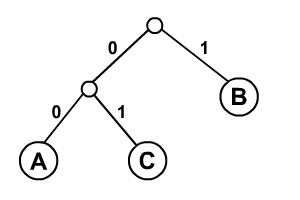
\includegraphics[scale=0.5]{trie2.png}
\end{multicols}

Texto comprimido: \texttt{1.1.1.1.1.1.1.00.1.01}

\end{itemize}

\end{problems}

\end{document}